\documentclass[12pt, a4paper, lithuanian]{article}
\usepackage[utf8x]{inputenc}
\def\LTfontencoding{L7x}
\PrerenderUnicode{ąčęėįšųūž}
\usepackage[\LTfontencoding]{fontenc}
\usepackage[lithuanian]{babel}
\usepackage{VUMIFCS1bakalaurinis}
\usepackage{cite}
\usepackage{amsmath}
\usepackage{bm}
\usepackage{amsfonts}
\usepackage{float}
\usepackage{graphicx}
\usepackage{color}
\usepackage{listings}
\usepackage{wrapfig}
\usepackage{algpseudocode}
\usepackage{algorithm}
\usepackage{algorithmicx}
\usepackage{caption}
\usepackage{subfig}


% Titulinio aprašas
\vumifdept{Informatikos katedra}
\vumifpaper{Baigiamasis bakalauro darbas}
\title{Rizikų valdymo proceso modeliavimas}
\titleineng{Modeling of Risk Management Process}
\status{2 kurso 1 grupės studentas}
\author{Vardenis Pavardenis}
% \secondauthor{Vardonis Pavardonis}
\supervisor{doc. dr. Vardaitis Pavardaitis}
\reviewer{dr. Vardauskas Pavardauskas}
\date{Vilnius\\ \the\year}

\begin{document}
\maketitle

\tableofcontents

\sectionnonum{Santrumpos}
Šiame skyriuje pateikiamas sutartinių ženklų, simbolių, vienetų ir terminų sutrumpinimų
sąrašas (jeigu ženklų, simbolių, vienetų ir terminų bendras skaičius didesnis
nei 10 ir kiekvienas iš jų tekste kartojasi daugiau nei po 3 kartus).

\sectionnonum{Įvadas}
Įvade apibūdinamas darbo tikslas, temos aktualumas ir siekiami rezultatai.

\section{Pagrindinė tiriamoji dalis}
Pagrindinėje tiriamojoje dalyje aptariama ir pagrindžiama tyrimo metodika;
pagal atitinkamas darbo dalis, nuosekliai, panaudojant lyginamosios analizės,
klasifikacijos, sisteminimo metodus bei apibendrinimus, dėstoma sukaupta ir
išanalizuota medžiaga.

\subsection{Poskyris}
Citavimo pavyzdys \cite{Banerjee1997}, \cite{EgArticle}.
% "`, "' - Lietuviškos kabutės 
\subsubsection{Skirsnis}
\subsubsubsection{Straipsnis}
\subsubsection{Skirsnis}
\section{Skyrius}
\subsection{Poskyris}
\subsection{Poskyris}

\sectionnonum{Išvados}
Išvadose ir pasiūlymuose, nekartojant atskirų dalių apibendrinimų,
suformuluojamos svarbiausios darbo išvados, rekomendacijos bei pasiūlymai.

\sectionnonum{Conclusions}
Šiame skyriuje pateikiamos išvados (reziume) anglų kalba.

\bibliography{bibliografija}   % Literatūros šaltiniai aprašomi bibliografija.bib faile

\appendix  % Priedai

\section{Niauroninio tinklo struktūra}
\begin{figure}[H]
    \centering
    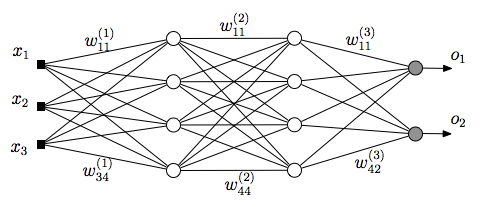
\includegraphics[scale=0.5]{img/MLP}
    \caption{Paveikslėlio pavyzdys}
    \label{img:mlp}
\end{figure}


\section{Eksperimentinio palyginimo rezultatai}
% tablesgenerator.com - converts calculators, e.g. excel, tables to LaTeX
\begin{table}[H]\footnotesize
  \centering
  \caption{Lentelės pavyzdys.}
  {\begin{tabular}{|l|c|c|} \hline
    Algoritmas & $\bar{x}$ & $\sigma^{2}$ \\
    \hline
    Algoritmas A  & 1.6335    & 0.5584       \\
    Algoritmas B  & 1.7395    & 0.5647       \\
    \hline
  \end{tabular}}
  \label{tab:table example}
\end{table}

\end{document}
